\documentclass[compress]{beamer}
\usetheme{Antibes}
\usecolortheme{dolphin}
\usefonttheme[onlymath]{serif}

\usepackage{amsmath}
\usepackage{mathcomp}
\usepackage[utf8]{inputenc}
\usepackage{graphicx}
\graphicspath{{./images/}}
\usepackage{listings}
\usepackage{caption}
\usepackage{url}
\usepackage[backend=biber,style=trad-abbrv]{biblatex}

\bibliography{literature}

\usepackage{tikz}
\usetikzlibrary{automata,positioning}

\title{Checking Equivalence of Nondeterministic Finite Automata}
\author{David Kofler}
\date{\today}
\institute{Master Seminar 2 \newline University of Innsbruck \newline Institute of Computer Science}


\begin{document}

\begin{frame}{}
	\maketitle
\end{frame}

\begin{frame}{}
	\tableofcontents
\end{frame}

\section{Deterministic finite automata}

\begin{frame}{Deterministic finite automata}
  \begin{block}{Definition}
    \begin{itemize}
      \item $M := (S, \Sigma, o, \delta)$
      \item $S$ and $\Sigma$ are finite sets
      \item $o : S \to \{\emptyset, \mathbf{\epsilon} \}$
      \item $\delta : S \to \Sigma \to S$
      \item $\mathcal{L} : S \to \mathcal{P}(\Sigma^\ast)$
    \end{itemize}
  \end{block}

  \begin{block}{Language Equivalence of DFA states}
    \begin{itemize}
      \item $\mathcal{L}(x) = o(x) \cup \bigcup_{a \in A}{\mathcal{L}({\delta(x, a)})}$
      \item $x_1 \sim x_2 \Leftrightarrow \mathcal{L}(x_1) = \mathcal{L}(x_2)$
    \end{itemize}
  \end{block}
\end{frame}

\begin{frame}{Example}
  \begin{figure}
    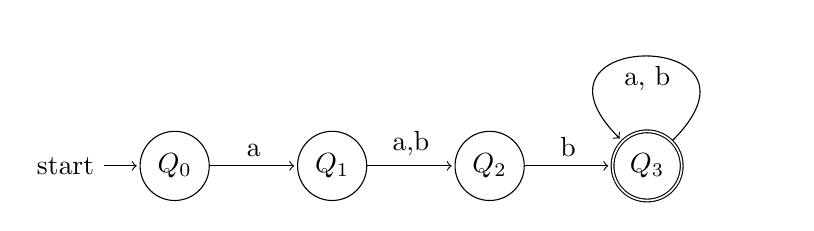
\begin{tikzpicture}[shorten >=1pt,node distance=2cm,on grid,auto]
      \node[state,initial] (q_0) [] {$Q_0$};
      \node[state] (q_1) [right=of q_0] {$Q_1$};
      \node[state] (q_2) [right=of q_1] {$Q_2$};
      \node[state,accepting] (q_3) [right=of q_2] {$Q_3$};
        \path[->]
        (q_0) edge node {a} (q_1)
        (q_1) edge node {a,b} (q_2)
              %edge node [below] {b} (q_2)
        (q_2) edge node {b} (q_3)
        (q_3) edge [loop] node {a, b} ();
    \end{tikzpicture}
  \end{figure}
\end{frame}

\begin{frame}{Proving language equivalence}
  \begin{block}{Bisimulations}
    \begin{itemize}
      \item Relation between states: $\doteqdot \subseteq S \times S$
      \item $\doteqdot \text{ is bisimulation } \Leftrightarrow x_1 \doteqdot x_2 \Rightarrow $
        \begin{itemize}
          \item $o(x) = o(y)$, and
          \item $\forall a \in \Sigma: \delta(x_1, a) \doteqdot \delta(x_2, a)$
        \end{itemize}
    \end{itemize}
   \end{block}

   \begin{block}{Language equivalence}
     Coinduction:
     $\mathcal{L}(x_1) = \mathcal{L}(x_2) \Leftrightarrow \exists$ bisimulation $\doteqdot: x_1 \doteqdot x_2$
   \end{block}
\end{frame}

\section{Nondeterministic finite automata}

\begin{frame}{Nondeterministic finite automata}
  \begin{block}{Definition}
    \begin{itemize}
      \item $N := (S, \Sigma, o, \delta)$
      \item $S$ and $\Sigma$ are finite sets
      \item $o : S \to \{\emptyset, \mathbf{\epsilon} \}$,
            $\delta : S \to \Sigma \to \mathcal{P}(S)$
      \item $\mathcal{L} : S \to \mathcal{P}(\Sigma^\ast)$
    \end{itemize}
  \end{block}
\end{frame}

\begin{frame}{Determinisation by powerset construction}
  %\begin{block}{Powerset construction}
    %\begin{itemize}
      \begin{align}
        o^\#(X) = &\begin{cases}
            o(x)                    &\text{ if } X = \{x\}, x \in S\\
            \emptyset               &\text{ if } X = \emptyset\\
            o^\#(X_1) \cup o^(X_2)  &\text{ if } X = X_1 \cup X_2\\
          \end{cases}\\
        \delta^\#(X, a) = &\begin{cases}
            \delta(x, a)                              &\text{ if } X =\{x\}, x \in S\\
            \emptyset                                 &\text{ if } X = \emptyset\\
            \delta^\#(X_1, a) \cup \delta^\#(X_2, a)  &\text{ if } X = X_1 \cup X_2\\
          \end{cases}
      \end{align}
    %\end{itemize}
  %\end{block}

  \begin{block}{Determinised NFA}
    We obtain the determinised automaton $N^\# = (\mathcal{P}(S), \Sigma, o^{\#}, d^{\#})$
      from the NFA $N = (S, \Sigma, o, \delta)$
  \end{block}
\end{frame}

\begin{frame}{Language equivalence}
  \begin{block}{Bisimulations on sets of states}
    \begin{itemize}
      \item Relation between sets of states: $\doteqdot \subseteq \mathcal{P}(S) \times \mathcal{P}(S)$
      \item $\doteqdot$ is bisimulation $\Leftrightarrow \forall X_1, X_2 \in \mathcal{P}(S): $
        \begin{itemize}
          \item $o^\#(X_1) = o^\#(X_2)$, and
          \item $\forall a \in \Sigma: \delta^\#(X_1, a) \doteqdot \delta^\#(X_2, a)$
        \end{itemize}
    \end{itemize}
  \end{block}

  \begin{block}{Language equivalence}
    \begin{itemize}
      \item $x_1 \sim x_2 \Leftrightarrow \mathcal{L}(\{x_1\}) = \mathcal{L}(\{x_2\})$
      \item Coinduction:\\
        $\mathcal{L}(X_1) = \mathcal{L}(X_2) \Leftrightarrow \exists$ bisimulation $\doteqdot^\#: X_1 \doteqdot^\# X_2$
    \end{itemize}
  \end{block}
\end{frame}

\subsection{Lattice structure of Determinsed NFA}

\begin{frame}{Lattices}
  \begin{block}{Lower Semi-Lattice}
    \begin{itemize}
      \item Set $X$ with operation $+: X \to X \to X$
      \item $+$ is associative and commutative
      \item $\forall x \in X: x + x = x$, $\exists 0_X \in X: \forall x \in X: x + 0_X = x$
      \item $f: X \to X$ homomorphism $\Leftrightarrow f(0_X) = 0_X $\\
            and $\forall x, y \in X: f(x+y) = f(x) + f(y)$
    \end{itemize}
  \end{block}
\end{frame}

\begin{frame}{States of Determinised NFA}
  \begin{itemize}
    \item Determinised NFA: $M^\# = (\mathcal{P}(S), \Sigma, o^\#, \delta^\#)$
    \item $o^\#$ and $\delta^\#$ are homomorphisms
    \item $\mathcal{L}$ is also a homomorphism
    \item $\mathcal{L}(X \cup Y) = \mathcal{L}({X}) \cup \mathcal{L}({Y})$
  \end{itemize}
\end{frame}

\section{Computing bisimulations}

\begin{frame}{Naive algorithm}
  \begin{align*}
    \underline{Naive(x, y)}: &\quad S \to S \to \{true, false\} \\
    \text{(1) } & R := \emptyset, todo := \emptyset;\\
    \text{(2) } & todo := todo \cup \{(x, y)\};\\
    \text{(3) } & \text{while } todo \neq \emptyset \text{ do}\\
      & \text{(3.1)}\quad todo := todo \setminus (x', y');\\
      & \text{(3.2)}\quad \text{if } (x', y') \in R \text{ then goto (3)};\\
      & \text{(3.3)}\quad \text{if } o(x') \neq o(y) \text{ then return } false;\\
      & \text{(3.4)}\quad todo := todo \cup \bigcup_{a \in \Sigma}{(\delta(x', a), \delta(y', a))} \\
      & \text{(3.5)}\quad R := R \cup \{(x', y')\} \\
    \text{(4) } & \text{return } true;\\
  \end{align*}
\end{frame}

\begin{frame}{Comments}
  \begin{itemize}
    \item The Algorithm terminates since $\mathcal{P}(S)$ is finite
    \item The algorithm is similar for $(\mathcal{P}(S), \Sigma, o^\#, \delta^\#)$
    \item Statement (3.2) is essential for optimisation:\\
      \begin{itemize}
        \item $\text{(3.2)}\quad \text{if } (x', y') \in R \text{ then goto (3)};$
        \item $(x', y') \in R$ can be replaced by $(x', y') \in f(R)$
        \item $f$ has to be $compatible$
      \end{itemize}
  \end{itemize}
\end{frame}

\section{Optimizations}

\begin{frame}{Compatibility}
  \begin{block}{Progression}
    \begin{itemize}
      %\item $R, R' \subseteq S \times S$
      \item $R \rightarrowtail R' \Leftrightarrow \forall (x, y) \in R:$\\
        \begin{itemize}
          \item $o(x) = o(y)$, and
          \item $\forall a \in \Sigma: (\delta(x, a), \delta(y, a)) \in R'$
        \end{itemize}
      %\item $R \rightarrowtail R \Leftrightarrow R \text{ is bisimulation}$
    \end{itemize}
  \end{block}

  \begin{block}{Compatibility}
    $f : (S \times S) \to (S \times S)$ is compatible iff \\
    \begin{itemize}
      \item $f$ monotone: $\forall R: R \subseteq f(R)$, and
      \item $f$ preserves $\rightarrowtail$:
        $R \rightarrowtail R' \Rightarrow f(R) \rightarrowtail f(R')$
    \end{itemize}
  \end{block}
\end{frame}

\begin{frame}{Optimizations}
  \begin{block}{Compatible functions}
    \begin{itemize}
      \item $id, f \circ g, \cup F, f^\omega$
      \item Symmetric ($s$), reflexive ($r$) and transitive closure ($t$)
      \item Equivalence closure: $e = (s \cup r \cup t \cup id)^\omega$
    \end{itemize}
  \end{block}

  \begin{block}{Optimization}
    \begin{itemize}
      \item $R$ is bisimulation if $R \rightarrowtail R$
      \item $R$ is bisimulation up to $f$ if $R \rightarrowtail f(R)$
      \item If $f$ is compatible, hence monotone, $|R| \leq |f(R)|$ !
    \end{itemize}
  \end{block}
\end{frame}

\begin{frame}{Algorithms}
  \begin{itemize}
    \item Naive algorithm: Builds a bisimulation
    \item Hopcroft and Karp's algorithm\cite{hopcroft1971linear}: Bisimulation up to equivalence
    \item Contribution of Filippo Bonchi and Damien Pous\cite{bonchi2013checking}:
      Bisimulation up to congruence ($c : \mathcal{P}(S)^2 \to \mathcal{P}(S)^2)$):\\
        \begin{align}
          u(\text{R}) &= \{(X_1 \cup X_2, Y_1 \cup Y_2) | X_1 \text{ R } Y_1, X_2 \text{ R } Y_2\}\\
          u&\text{ is monotone and preserves }\rightarrowtail\\
          c &= (s \cup r \cup t \cup id \cup u)^\omega
        \end{align}
    \item Antichain algorithms
      \cite{doyen2010antichain}\cite{abdulla2010simulation}\cite{lengal2012vata}:
      simulation up to upward closure
  \end{itemize}
\end{frame}

\section{Experimental Results}

\section{Conclusion}

\begin{frame}{Main Takeaways}
  \begin{itemize}
    \item Naive algorithm, ACs, HK, HKC, and other variants can be uniformely
      presented by using bisimulations.
    \item The AC algorithms perform astonishingly bad
      \begin{itemize}
        \item Maybe \textbf{libvata} is not optimized for string automata
      \end{itemize}
  \end{itemize}
\end{frame}

\end{document}
